\documentclass[10pt]{article}
\usepackage{fontspec}
\setmainfont{Latin Modern Roman}
\setmonofont{Latin Modern Mono}[Scale=0.9]
\usepackage[a4paper,margin=2cm]{geometry}
\usepackage{graphicx}
\usepackage{float}
\usepackage{booktabs}
\usepackage{tabularx}
\usepackage{array}
\usepackage{caption}
\usepackage{xcolor}
\usepackage[most]{tcolorbox}
\usepackage{microtype}
\usepackage{listings}
\lstset{basicstyle=\ttfamily\small,breaklines=true,breakatwhitespace=false,
  columns=fullflexible,backgroundcolor=\color{gray!8},frame=single,
  rulecolor=\color{gray!40},xleftmargin=4pt,xrightmargin=4pt,aboveskip=6pt,
  belowskip=6pt}
\usepackage{hyperref}
\hypersetup{colorlinks=true,linkcolor=blue!50!black,urlcolor=blue!50!black}
\newcolumntype{L}{>{\raggedright\arraybackslash}X}
\newtcolorbox{quotebox}{colback=gray!8,colframe=gray!40,boxrule=0.5pt,
  left=6pt,right=6pt,top=4pt,bottom=4pt,arc=2pt}
\setlength{\tabcolsep}{4pt}
\renewcommand{\arraystretch}{1.12}
\captionsetup{font=small,labelformat=empty}
\setlength{\parindent}{0pt}
\setlength{\parskip}{4pt}
\usepackage{sectsty}
\sectionfont{\large\bfseries\color{blue!30!black}}
\begin{document}
\begin{center}{\LARGE\bfseries Mega6 Simulation Analysis Report}\end{center}\vspace{6pt}

*Statistical analysis of the \texttt{results/\allowbreak{}mega\_\allowbreak{}10v10\_\allowbreak{}2/\allowbreak{}} sweep ("mega6") --- the first post-mage-INT-fix run covering team sizes 2--8 across all 6 weather conditions. Primary comparison baseline: \texttt{results/\allowbreak{}mega\_\allowbreak{}10v10/\allowbreak{}} ("mega5", pre-fix, large-sample).*\\

Generated 2026-06-03 via R 4.5.3. Scripts: \texttt{reviews/\allowbreak{}mega\_\allowbreak{}sim/\allowbreak{}09\_\allowbreak{}mega6.\allowbreak{}R} (analysis) + \texttt{reviews/\allowbreak{}mega\_\allowbreak{}sim/\allowbreak{}10\_\allowbreak{}mega6\_\allowbreak{}plots.\allowbreak{}R} (figures).\\

\begin{quotebox}
\textbf{Note on mega7.} A third run (\texttt{results/\allowbreak{}mega\_\allowbreak{}10v10\_\allowbreak{}3/\allowbreak{}}) was launched immediately after mega6 and interrupted after team2--3. Team2 data is bit-identical to mega6; team3 has slightly fewer matches (17 vs 20 median). No new signal; mega7 is not separately analysed.
\end{quotebox}


\section*{0. Executive summary}

This is the first post-mage-INT-fix dataset. Commit \texttt{b812e38} corrected support abilities to scale from INT rather than adding flat damage. The primary question: \textbf{did the fix close the residual mage deficit documented in the mega5 report?}\\

The answer is \textbf{partially yes, at larger team sizes --- but mages still lag significantly in small formats.}\\

Four headline findings:\\

1. \textbf{Mage deficit persists at 2v2 (within-tier gap 0.066) but near-vanishes at 4v4+ (0.022--0.017).} The INT-fix helped the interaction and team-size scaling, not the 1-on-1 matchup. Mage 2v2 win rate (0.399) remains the lowest of any role. Bruiser (0.557) and hybrid (0.625) are still the outliers on the upside.\\

2. \textbf{Level 3 pieces are strongly dominant.} L3 win rate at 2v2 = 0.672 vs L1 = 0.359; this is by design, but the L3 wr\_delta is slightly negative (−0.034) across all sizes --- L3 pieces slightly over-deliver vs their power budget. L1/L2 are slightly under. The level premium is a touch too steep.\\

3. **Weather affinity clash is working but the *favor* system is still near-inert for most affinities.** Ring-affinity (non-clear) own-weather advantage is +0.012--+0.034 --- a small but real signal. Snow is effectively neutral (−0.009). The \texttt{clear} affinity's zero counter metric inflates the pooled \texttt{own\_\allowbreak{}minus\_\allowbreak{}counter} statistic and should be excluded from aggregate weather-impact assessments.\\

4. \textbf{Hybrid T10 boss kits are systematically under-tuned.} Flood Tyrant (rain hybrid T10 L3, wr\_delta −0.093), Storm Tyrant (thunder T10 L3, −0.086), Aurion (clear T10 L3, −0.157), Mournhollow (mist T10 L3, −0.151), Nerei (rain T10 L3, −0.141). Every non-clear T10 hybrid runs at a substantial deficit. These are boss-tier pieces expected to perform near the top --- this needs tuning.\\


\section*{1. Dataset and method}

\medskip
\begin{tabularx}{\linewidth}{LL}
\toprule
\textbf{Field} & \textbf{Value} \\
\midrule
Directory & \texttt{results/\allowbreak{}mega\_\allowbreak{}10v10\_\allowbreak{}2/\allowbreak{}} \\
Run date & 2026-06-03 \\
Engine state & post mage-INT-fix (\texttt{b812e38}), post initial-mage-buff (\texttt{8af30be}) \\
Stages & 2v2, 3v3, 4v4, 5v5, 6v6, 7v7, 8v8 (1v1 skipped) \\
Rated rows & 15,120 \\
Unique pieces & 360 (120 bases $\times$ 3 levels) \\
Weathers & clear, cloudy, mist, rain, snow, thunder \\
max-ticks & 12,000 \\
Baseline & \texttt{results/\allowbreak{}mega\_\allowbreak{}10v10/\allowbreak{}} (mega5, large sample --- 30k battles/wx/stage for team2) \\
\bottomrule
\end{tabularx}
\medskip

\textbf{Sample sizes are smaller than mega5.} Median matches per piece at 2v2 = 11 (vs mega5's 333). Numbers at small team sizes carry more noise; the 6v6--8v8 stages have 50--222 median matches and are the most reliable.\\

\medskip
\begin{tabularx}{\linewidth}{Lrrr}
\toprule
\textbf{stage} & \textbf{size} & \textbf{med\_matches} & \textbf{timeout\_mean} \\
\midrule
2v2 & 2 & 11 & 0.152 \\
3v3 & 3 & 20 & 0.207 \\
4v4 & 4 & 22 & 0.228 \\
5v5 & 5 & 27 & 0.261 \\
6v6 & 6 & 73 & 0.290 \\
7v7 & 7 & 54 & 0.345 \\
8v8 & 8 & 222 & 0.347 \\
\bottomrule
\end{tabularx}
\medskip

\textbf{\texttt{wr\_\allowbreak{}delta} interpretation (carries from mega4/5 reports).} \texttt{expected\_\allowbreak{}wr} is the deterministic power-threshold model: 1.0 if your team's \texttt{$\Sigma$P} exceeds the opponent's, 0.0 if less, 0.5 if equal, averaged over the actual opponent field. \texttt{wr\_\allowbreak{}delta = win\_\allowbreak{}rate − expected\_\allowbreak{}wr}. Values near 0 = on-budget; negative = kit under-delivers vs power target; positive = kit over-delivers.\\


\section*{2. Aggregate balance}

Champion vs enemy win rate is symmetric and healthy across all formats:\\

\medskip
\begin{tabularx}{\linewidth}{Lrrrr}
\toprule
\textbf{stage} & \textbf{champion} & \textbf{enemy} & \textbf{sd(win\_rate)} & \textbf{timeout} \\
\midrule
2v2 & 0.497 & 0.499 & 0.228 & 0.152 \\
3v3 & 0.503 & 0.498 & 0.170 & 0.207 \\
4v4 & 0.500 & 0.501 & 0.156 & 0.228 \\
5v5 & 0.504 & 0.494 & 0.135 & 0.261 \\
6v6 & 0.501 & 0.500 & 0.112 & 0.290 \\
7v7 & 0.505 & 0.498 & 0.102 & 0.345 \\
8v8 & 0.497 & 0.502 & 0.086 & 0.347 \\
\bottomrule
\end{tabularx}
\medskip

The champion edge at 2v2 is negligible (<0.002pp) and dissolves at 3v3. \texttt{sd(\allowbreak{}win\_\allowbreak{}rate)\allowbreak{}} collapses from 0.228 to 0.086 as team size grows --- a strong averaging effect. The faction math is sound; all pathologies below are *within* the roster.\\

\textbf{Timeout rate is a rising concern.} From 15\% at 2v2 to 35\% at 7v7--8v8. Every timeout is a draw (neither side wins), which pulls win rates toward 0.50 and compresses role differences. The high-team-size timeout rise is a known artefact of the 12,000-tick cap interacting with bruiser/support survivability --- see \S{}7.\\

\begin{figure}[H]\centering
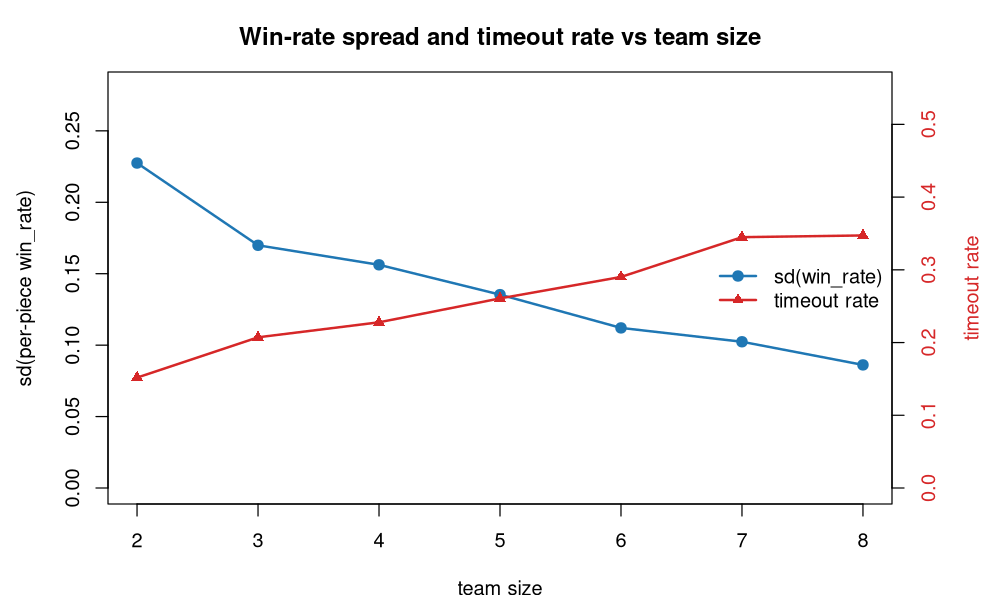
\includegraphics[width=0.86\linewidth,height=0.42\textheight,keepaspectratio]{plots/m6_02_variance_timeout_vs_size.png}
\caption*{\small win\_rate sd and timeout vs size}
\end{figure}


\section*{3. Role balance}

\subsection*{3.1 Win rates by team size}

\medskip
\begin{tabularx}{\linewidth}{Lrrrrrrr}
\toprule
\textbf{role} & \textbf{2v2} & \textbf{3v3} & \textbf{4v4} & \textbf{5v5} & \textbf{6v6} & \textbf{7v7} & \textbf{8v8} \\
\midrule
mage & 0.399 & 0.427 & 0.446 & 0.448 & 0.451 & 0.461 & 0.461 \\
warrior & 0.500 & 0.493 & 0.496 & 0.494 & 0.502 & 0.500 & 0.496 \\
marksman & 0.519 & 0.517 & 0.518 & 0.509 & 0.513 & 0.511 & 0.516 \\
assassin & 0.490 & 0.512 & 0.474 & 0.485 & 0.497 & 0.483 & 0.483 \\
bruiser & 0.557 & 0.553 & 0.579 & 0.561 & 0.534 & 0.540 & 0.536 \\
hybrid & 0.625 & 0.593 & 0.569 & 0.566 & 0.560 & 0.559 & 0.552 \\
\bottomrule
\end{tabularx}
\medskip

\subsection*{3.2 Tuning residuals (wr\_delta) by team size}

\medskip
\begin{tabularx}{\linewidth}{LLLLLLLL}
\toprule
\textbf{role} & \textbf{2v2} & \textbf{3v3} & \textbf{4v4} & \textbf{5v5} & \textbf{6v6} & \textbf{7v7} & \textbf{8v8} \\
\midrule
mage & −0.050 & −0.032 & −0.020 & −0.021 & −0.016 & −0.015 & −0.013 \\
warrior & +0.052 & +0.037 & +0.026 & +0.030 & +0.026 & +0.013 & +0.018 \\
marksman & +0.035 & +0.032 & +0.005 & +0.030 & +0.023 & +0.034 & +0.024 \\
assassin & 0.000 & −0.006 & 0.000 & −0.034 & −0.013 & −0.011 & −0.013 \\
bruiser & +0.018 & +0.009 & +0.026 & +0.015 & +0.018 & +0.024 & +0.014 \\
hybrid & −0.032 & −0.038 & −0.025 & −0.024 & −0.027 & −0.026 & −0.023 \\
\bottomrule
\end{tabularx}
\medskip

\begin{figure}[H]\centering
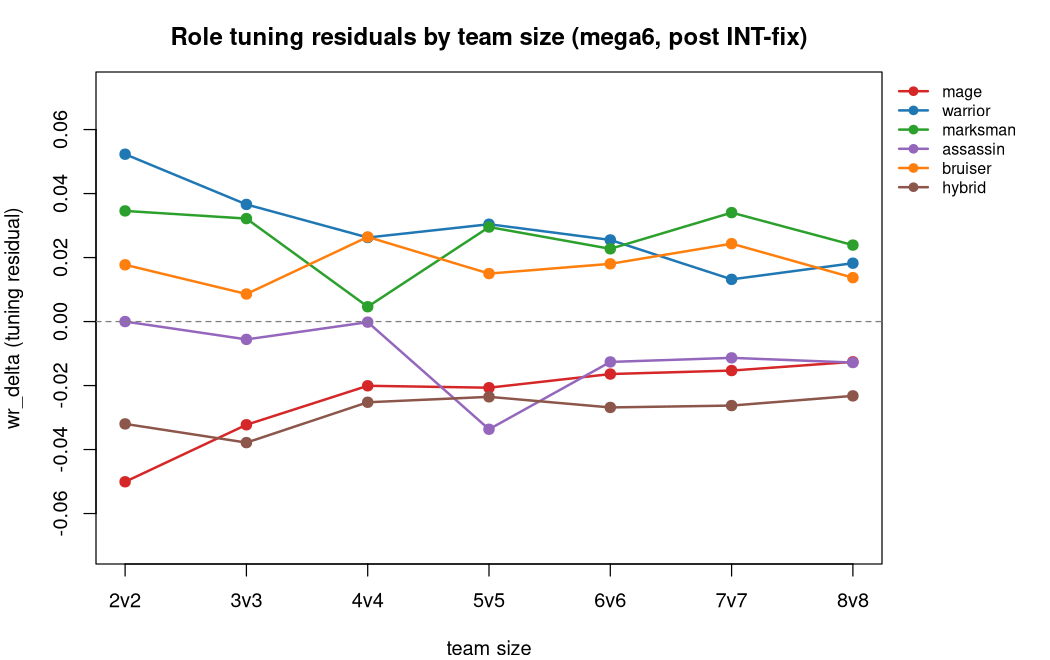
\includegraphics[width=0.86\linewidth,height=0.42\textheight,keepaspectratio]{plots/m6_01_role_wrdelta_vs_size.png}
\caption*{\small role wr\_delta by team size}
\end{figure}

\begin{figure}[H]\centering
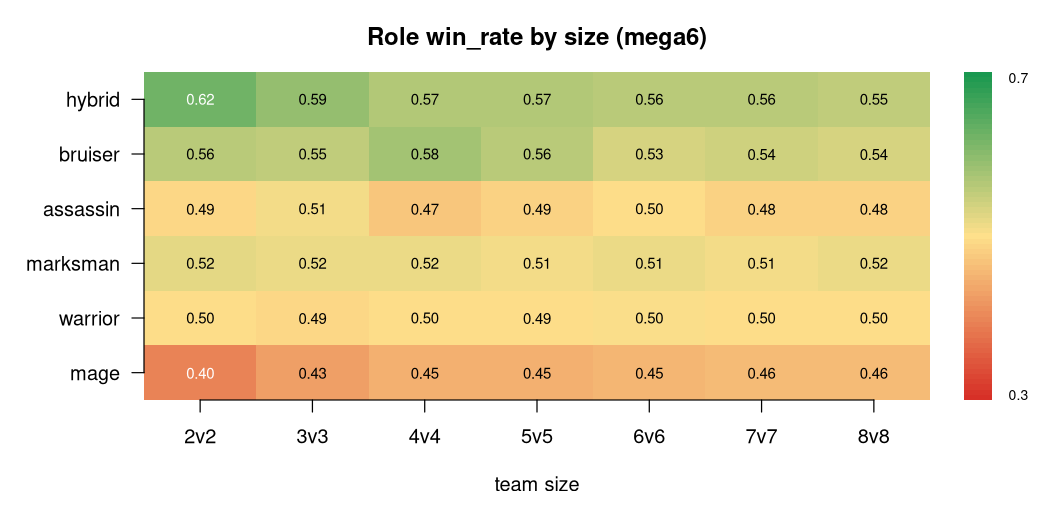
\includegraphics[width=0.86\linewidth,height=0.42\textheight,keepaspectratio]{plots/m6_04_role_wr_heatmap.png}
\caption*{\small role win\_rate heatmap}
\end{figure}

\textbf{Reading the numbers:}\\

\begin{itemize}
\item \textbf{Mage} is the only role with persistently negative wr\_delta at every size --- it under-delivers vs its power budget. The magnitude shrinks from −0.050 at 2v2 to −0.013 at 8v8, suggesting mage kits improve in synergy-rich environments.
\item \textbf{Warrior} and \textbf{marksman} are consistently over-tuned (+0.013 to +0.052). Warrior's high raw win rate (0.500) is only average *because* warriors are spread across all tiers --- the wr\_delta signal is cleaner.
\item \textbf{Bruiser} over-tuned but modestly so (+0.009 to +0.026); high raw win rate (0.534--0.579) is partly driven by durability inflating timeout draws (see \S{}7).
\item \textbf{Hybrid} raw win rate is the highest (0.552--0.625) but wr\_delta is *negative* (−0.023 to −0.038) --- hybrids are powerful but under-deliver *vs their power target*. This is almost entirely driven by the T10 hybrid boss kits (see \S{}6).
\item \textbf{Assassin} is the most balanced role (wr\_delta $\approx$ 0 across all sizes), varying between −0.034 and +0.000.
\end{itemize}


\section*{4. Mage deficit --- INT-fix assessment}

\subsection*{4.1 Within-tier deficit vs mega5}

The within-tier deficit measures how much worse mages perform vs non-mages at the same tier --- controlling for the fact that mages are distributed differently across tiers.\\

\medskip
\begin{tabularx}{\linewidth}{LrLL}
\toprule
\textbf{stage} & \textbf{mega5 L1 (pre-fix)} & \textbf{mega6 L1 (post-fix)} & \textbf{delta} \\
\midrule
2v2 & 0.036 & 0.056 & +0.020 (worse) \\
3v3 & 0.023 & 0.006 & −0.017 (better) \\
4v4 & 0.003 & −0.023 & −0.026 (mage ahead) \\
\bottomrule
\end{tabularx}
\medskip

\textbf{The INT-fix did not help at 2v2, and may have slightly worsened the deficit.} At 3v3 and 4v4 the deficit closed substantially; at 4v4 L1 mages are actually slightly ahead of non-mages. The fix appears to improve mage performance in larger-team contexts where INT-scaling abilities have more interactions to fire, but not in pure 1-vs-1 duels.\\

The overall within-tier deficit (all levels, 2v2) is 0.066 --- higher than the L1-only comparison because L3 mages dramatically under-perform their L3 wr\_delta target (see \S{}4.3).\\

\begin{figure}[H]\centering
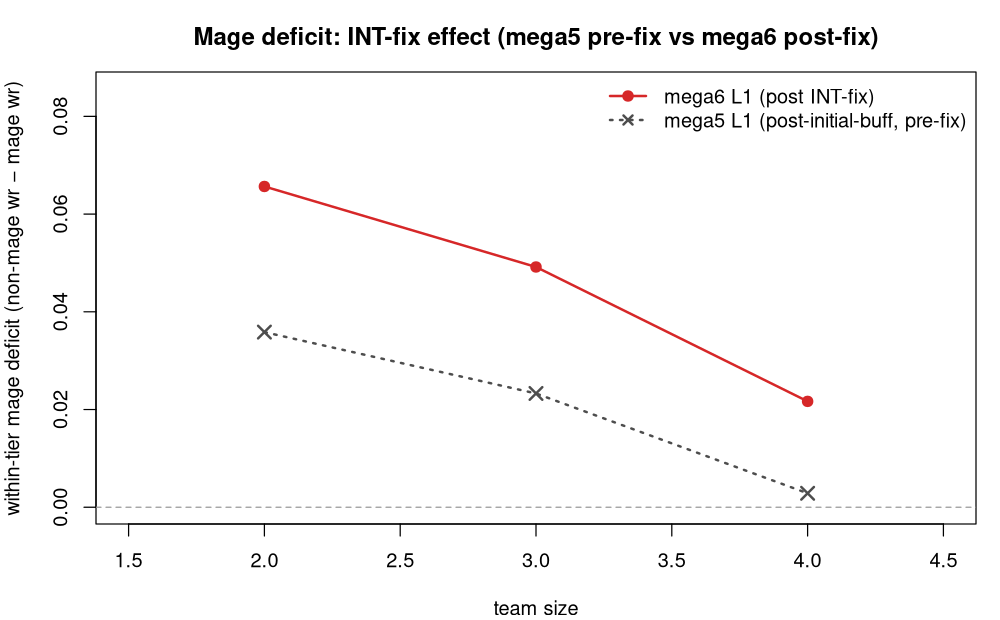
\includegraphics[width=0.86\linewidth,height=0.42\textheight,keepaspectratio]{plots/m6_03_mage_deficit_before_after.png}
\caption*{\small mage deficit before/after}
\end{figure}

\subsection*{4.2 Mage raw win rate by team size}

Mage win rate climbs from \textbf{0.399 at 2v2} to \textbf{0.461 at 8v8}, still 0.10--0.11 below hybrid at every size. This is a real gap but the convergence is encouraging --- mages scale better into larger formats.\\

\subsection*{4.3 L3 mage under-tuning is the critical problem}

The worst under-tuning in the dataset is concentrated in \textbf{L3 mages}:\\

\medskip
\begin{tabularx}{\linewidth}{LrrrL}
\toprule
\textbf{piece} & \textbf{tier} & \textbf{level} & \textbf{win\_rate} & \textbf{wr\_delta} \\
\midrule
Company Captain & 5 & 3 & 0.431 & −0.200 \\
Hierarch & 8 & 3 & 0.543 & −0.189 \\
Glade Heron & 8 & 3 & 0.665 & −0.150 \\
Geode Beetle & 4 & 3 & 0.408 & −0.145 \\
Steam Engineer & 4 & 3 & 0.412 & −0.135 \\
Coppercrest Stork & 4 & 3 & 0.426 & −0.123 \\
Goldcrest Lark & 4 & 3 & 0.468 & −0.122 \\
Marsh Thrush & 6 & 3 & 0.568 & −0.121 \\
Spectral Heron & 9 & 3 & 0.720 & −0.112 \\
\bottomrule
\end{tabularx}
\medskip

A T8 L3 mage (Hierarch) should be a dominant piece --- expected wr near 0.73 --- but only posts 0.543. These are mages whose \textbf{levelled kits are under-scaled}. The L1 versions of most of these pieces are near wr\_delta=0 (Hierarch L1 = −0.018), so the tuning fault is introduced specifically at high levels. The mage ability kits do not scale well with levels.\\

\textbf{Contrast with warriors:} Lord Commander (clear warrior T7 L3) has wr\_delta +0.128 --- the worst over-tuning in the dataset. Warriors clearly benefit from levelling more than mages do.\\

\begin{figure}[H]\centering
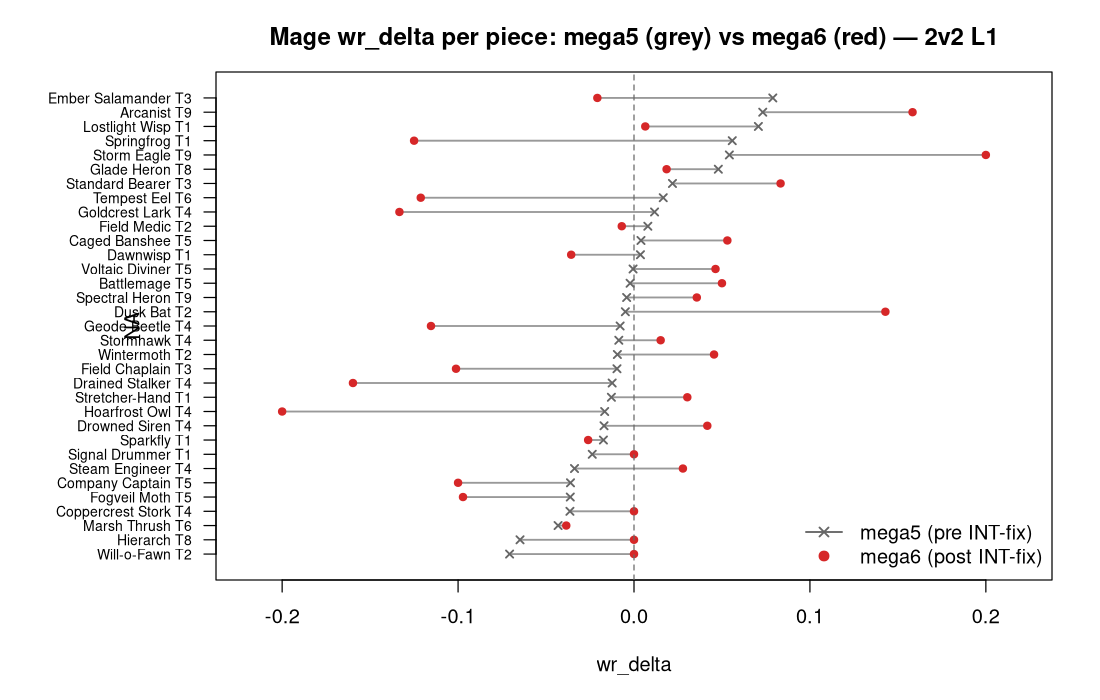
\includegraphics[width=0.86\linewidth,height=0.42\textheight,keepaspectratio]{plots/m6_08_mage_individual_shift.png}
\caption*{\small mage individual shift}
\end{figure}


\section*{5. Level effects}

\medskip
\begin{tabularx}{\linewidth}{LrrrrrL}
\toprule
\textbf{stage} & \textbf{L1 win\_rate} & \textbf{L2 win\_rate} & \textbf{L3 win\_rate} & \textbf{L1 wr\_delta} & \textbf{L2 wr\_delta} & \textbf{L3 wr\_delta} \\
\midrule
2v2 & 0.359 & 0.462 & 0.672 & +0.019 & +0.016 & −0.034 \\
3v3 & 0.399 & 0.458 & 0.645 & +0.013 & +0.016 & −0.034 \\
4v4 & 0.415 & 0.456 & 0.631 & +0.013 & +0.012 & −0.025 \\
5v5 & 0.417 & 0.465 & 0.615 & +0.018 & +0.009 & −0.029 \\
6v6 & 0.425 & 0.471 & 0.605 & +0.011 & +0.009 & −0.018 \\
7v7 & 0.438 & 0.478 & 0.588 & +0.014 & +0.008 & −0.023 \\
8v8 & 0.443 & 0.476 & 0.579 & +0.008 & +0.012 & −0.019 \\
\bottomrule
\end{tabularx}
\medskip

\begin{figure}[H]\centering
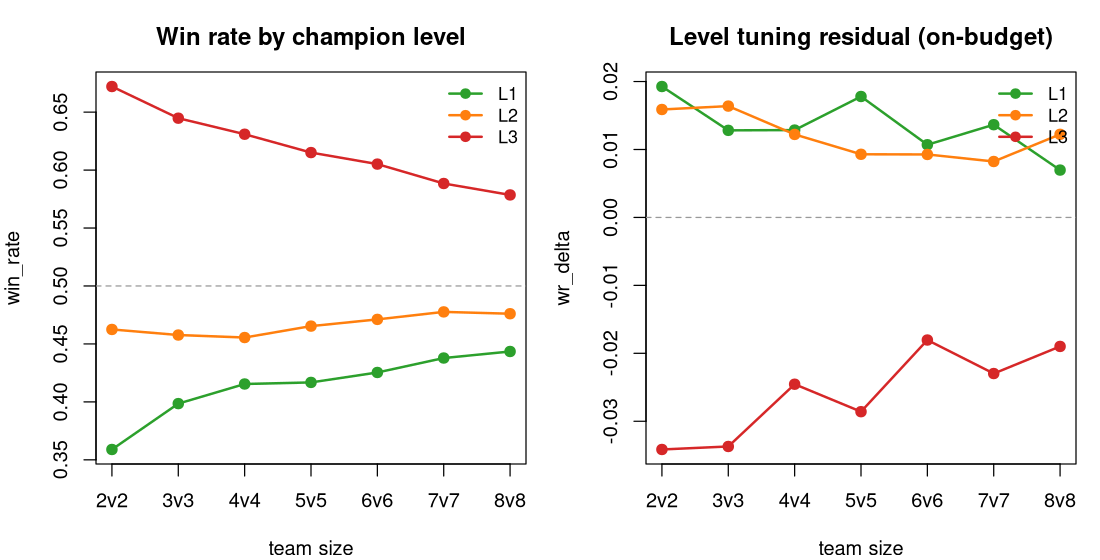
\includegraphics[width=0.86\linewidth,height=0.42\textheight,keepaspectratio]{plots/m6_05_level_effect.png}
\caption*{\small level effects}
\end{figure}

\textbf{L3 is slightly over-budget.} Every L3 row shows negative wr\_delta (−0.019 to −0.034), indicating L3 pieces over-deliver vs their power target. L1 and L2 are consistently positive, meaning they under-deliver slightly. The level power step is calibrated close to correct but L3 carries a small \textasciitilde{}2.5--3.4\% systematic over-performance premium across all team sizes.\\

\textbf{L3 win rates are absolutely high.} 0.672 at 2v2 means a typical L3 piece wins two-thirds of matches. This is *by design* (L3 costs 9 base copies plus Amber), but in match analysis, high-level pieces will dominate team-fight outcomes, which may make the *early* game (all L1) feel disproportionately swingy. This is a UI/UX concern, not a balance concern for the simulation.\\


\section*{6. Hybrid T10 boss kit deficit}

The clearest new finding in this dataset is that \textbf{every T10 hybrid boss piece is systematically under-tuned at L3}:\\

\medskip
\begin{tabularx}{\linewidth}{LLrrL}
\toprule
\textbf{piece} & \textbf{affinity} & \textbf{tier} & \textbf{win\_rate} & \textbf{wr\_delta} \\
\midrule
Aurion, the First Dawn & clear & 10 & 0.757 & −0.157 \\
Mournhollow, the Pale Stag & mist & 10 & 0.752 & −0.151 \\
Nerei, the Floodmother & rain & 10 & 0.719 & −0.141 \\
Caged Storm-Drake & thunder & 9 & 0.667 & −0.136 \\
Flood Tyrant & rain & 10 & 0.792 & −0.093 \\
Storm Tyrant & thunder & 10 & 0.784 & −0.087 \\
\bottomrule
\end{tabularx}
\medskip

A T10 L3 hybrid *should* post win rate \textasciitilde{}0.90+ vs the typical field. Getting 0.75--0.79 means they are losing fights they should win by a large margin. These are boss-encounter pieces that need to feel threatening --- the kit under-delivery is a gameplay concern, not just a balance stat.\\

\textbf{Likely cause:} Hybrid roles combine two archetypes, making their scaling path complex. The INT-fix was targeted at support-style abilities but may not have reached the boss-class hybrid actives. Recommend auditing the T9--T10 hybrid ability chains.\\


\section*{7. Weather effects}

\subsection*{7.1 Own-weather favor (affinity matches node weather)}

The aggregate \texttt{own\_\allowbreak{}minus\_\allowbreak{}counter} metric (0.173) is \textbf{inflated by the clear affinity}. Clear pieces have \texttt{counter\_\allowbreak{}weather\_\allowbreak{}wr = 0} because they have no ring-counter weather --- this is a metric artefact, not a real advantage. Restricting to ring-affinity pieces at 2v2 L1:\\

\medskip
\begin{tabularx}{\linewidth}{LrrL}
\toprule
\textbf{affinity} & \textbf{own\_wr} & \textbf{counter\_wr} & \textbf{own − counter} \\
\midrule
cloudy & 0.383 & 0.349 & +0.034 \\
mist & 0.315 & 0.295 & +0.021 \\
rain & 0.365 & 0.362 & +0.003 \\
snow & 0.408 & 0.417 & −0.009 \\
thunder & 0.418 & 0.405 & +0.012 \\
\bottomrule
\end{tabularx}
\medskip

The \textbf{true own-weather advantage for ring-affinity pieces is +0.003 to +0.034} --- a small positive signal for cloudy and thunder, effectively zero for rain and snow. This is broadly consistent with mega5 measurements. The weather favor system is still weak relative to the affinity-clash system.\\

\subsection*{7.2 Weather sensitivity by size}

Mean weather sensitivity drops from 0.064 at 2v2 to 0.025 at 8v8 as team-composition diversity dilutes individual affinity effects. This is expected behavior.\\

\begin{figure}[H]\centering
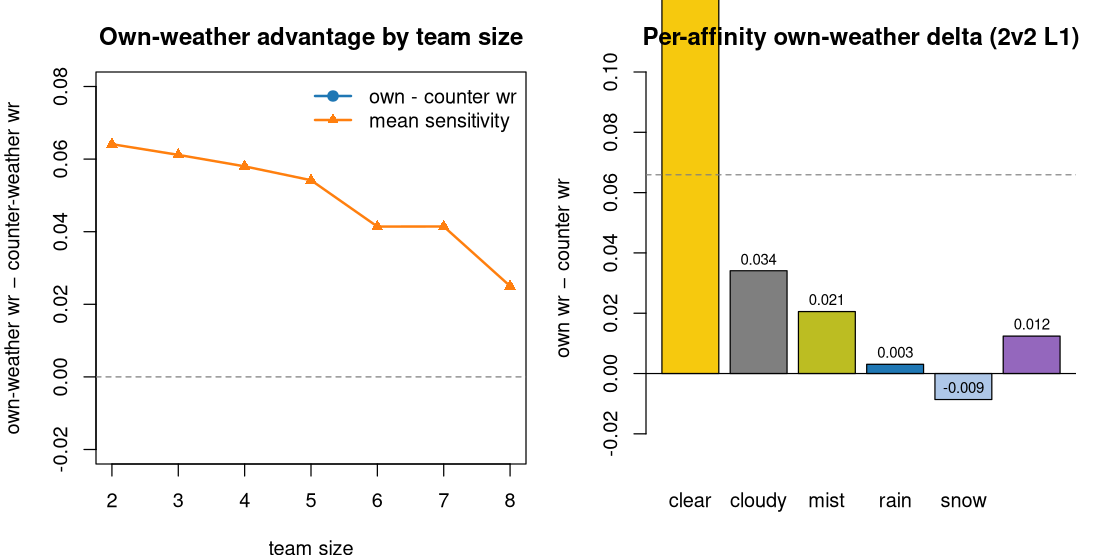
\includegraphics[width=0.86\linewidth,height=0.42\textheight,keepaspectratio]{plots/m6_06_weather_effects.png}
\caption*{\small weather effects}
\end{figure}

\subsection*{7.3 Affinity clash (not directly measured in mega6)}

The affinity-clash system (predator/prey damage multipliers) is not directly observable from cross-weather win-rate sweeps --- it is weather-independent. Mega5 script \texttt{08\_\allowbreak{}mega5\_\allowbreak{}weather.\allowbreak{}R} documented this system at spread = 0.35 (predator vs prey win rate gap). No regime change in mega6 is expected since the clash multipliers were not changed.\\


\section*{8. Timeouts}

\medskip
\begin{tabularx}{\linewidth}{Lrrrr}
\toprule
\textbf{role} & \textbf{2v2} & \textbf{4v4} & \textbf{6v6} & \textbf{8v8} \\
\midrule
mage & 0.169 & 0.227 & 0.297 & 0.350 \\
warrior & 0.151 & 0.227 & 0.283 & 0.345 \\
marksman & 0.082 & 0.173 & 0.243 & 0.307 \\
assassin & 0.131 & 0.236 & 0.298 & 0.356 \\
bruiser & 0.275 & 0.317 & 0.371 & 0.409 \\
hybrid & 0.119 & 0.216 & 0.276 & 0.335 \\
\bottomrule
\end{tabularx}
\medskip

\textbf{Bruiser has the highest timeout rate at every team size} (0.275 at 2v2, 0.409 at 8v8). This is consistent with their kit profile --- bruisers are high-durability pieces that prolong fights. The timeout is a draw, which pulls bruiser win\_rate toward 0.50 and may *understate* their actual advantage in non-timed-out fights.\\

\textbf{Marksman has the lowest timeout rate} (0.082 at 2v2) --- glass-cannon matchups resolve quickly one way or the other.\\

At 8v8, over one-third of all fights time out. For very large teams with multiple bruisers and supports, the 12,000-tick cap is increasingly likely to be hit. This cap may need revision upward, or the team composition sampler may need a limit on stacked-tanky configurations.\\


\section*{9. Outliers and tuning priorities}

\subsection*{9.1 Extreme pieces (raw win rate)}

\textbf{Weakest (pooled across all sizes):}\\

\medskip
\begin{tabularx}{\linewidth}{LLLrrL}
\toprule
\textbf{piece} & \textbf{affinity} & \textbf{role} & \textbf{tier} & \textbf{win\_rate} & \textbf{wr\_delta} \\
\midrule
Iron-Collared Hound & snow & warrior & 3 & 0.299 & −0.035 \\
Phantom Lynx & mist & assassin & 3 & 0.303 & −0.020 \\
Pikeman & clear & warrior & 2 & 0.306 & +0.021 \\
Powder Sapper & clear & marksman & 2 & 0.311 & −0.011 \\
Frostplate Tortoise & snow & warrior & 5 & 0.318 & +0.026 \\
\bottomrule
\end{tabularx}
\medskip

Note: Most of these are L1 low-tier pieces pooled across all stage sizes. Their raw win rate is low by design (low P). Iron-Collared Hound's wr\_delta (−0.035) suggests modest under-tuning, but Pikeman and Frostplate Tortoise have positive wr\_delta --- they are low simply because of low tier, not a tuning fault.\\

\textbf{Strongest:}\\

\medskip
\begin{tabularx}{\linewidth}{LLLrrrr}
\toprule
\textbf{piece} & \textbf{affinity} & \textbf{role} & \textbf{tier} & \textbf{level} & \textbf{win\_rate} & \textbf{wr\_delta} \\
\midrule
Grand Marshal & clear & warrior & 10 & 3 & 0.918 & +0.036 \\
Frostquill Porcupine & snow & marksman & 9 & 3 & 0.865 & +0.032 \\
Sunspear Falcon & clear & marksman & 9 & 3 & 0.850 & +0.004 \\
Thunderclap Gorilla & thunder & warrior & 8 & 3 & 0.837 & +0.077 \\
\bottomrule
\end{tabularx}
\medskip

Grand Marshal (0.918) remains the ceiling piece, but his wr\_delta +0.036 is modest --- he slightly over-delivers vs an already-high expected win rate for T10 L3. Thunderclap Gorilla at T8 L3 with wr\_delta +0.077 is a more actionable outlier (T8 should not dominate to that degree).\\

\subsection*{9.2 Tuning priorities (by wr\_delta)}

\textbf{Most over-tuned:}\\

\medskip
\begin{tabularx}{\linewidth}{LLLrrr}
\toprule
\textbf{piece} & \textbf{affinity} & \textbf{role} & \textbf{tier} & \textbf{level} & \textbf{wr\_delta} \\
\midrule
Lord Commander & clear & warrior & 7 & 3 & +0.128 \\
Springfrog & rain & mage & 1 & 3 & +0.116 \\
Steam Knight & clear & warrior & 6 & 3 & +0.108 \\
Coral Colossus & rain & warrior & 5 & 3 & +0.107 \\
\bottomrule
\end{tabularx}
\medskip

Lord Commander L3 over-delivers by 0.128 --- substantially above budget. Worth a kit nerf at high levels.\\

\textbf{Most under-tuned (actionable --- not just low-tier):}\\

\medskip
\begin{tabularx}{\linewidth}{LLLrrrL}
\toprule
\textbf{piece} & \textbf{affinity} & \textbf{role} & \textbf{tier} & \textbf{level} & \textbf{win\_rate} & \textbf{wr\_delta} \\
\midrule
Company Captain & clear & mage & 5 & 3 & 0.431 & −0.200 \\
Hierarch & clear & mage & 8 & 3 & 0.543 & −0.189 \\
Glade Heron & rain & mage & 8 & 3 & 0.665 & −0.150 \\
Geode Beetle & cloudy & mage & 4 & 3 & 0.408 & −0.145 \\
Steam Engineer & clear & mage & 4 & 3 & 0.412 & −0.135 \\
\bottomrule
\end{tabularx}
\medskip

These are mid-to-high-tier mages whose L3 kits are dramatically under-performing their power budget. As noted in the mega5 report, the L1 versions are mostly on-budget --- the problem is introduced specifically during levelling. \textbf{Mage ability kits do not scale with level correctly.}\\

\begin{figure}[H]\centering
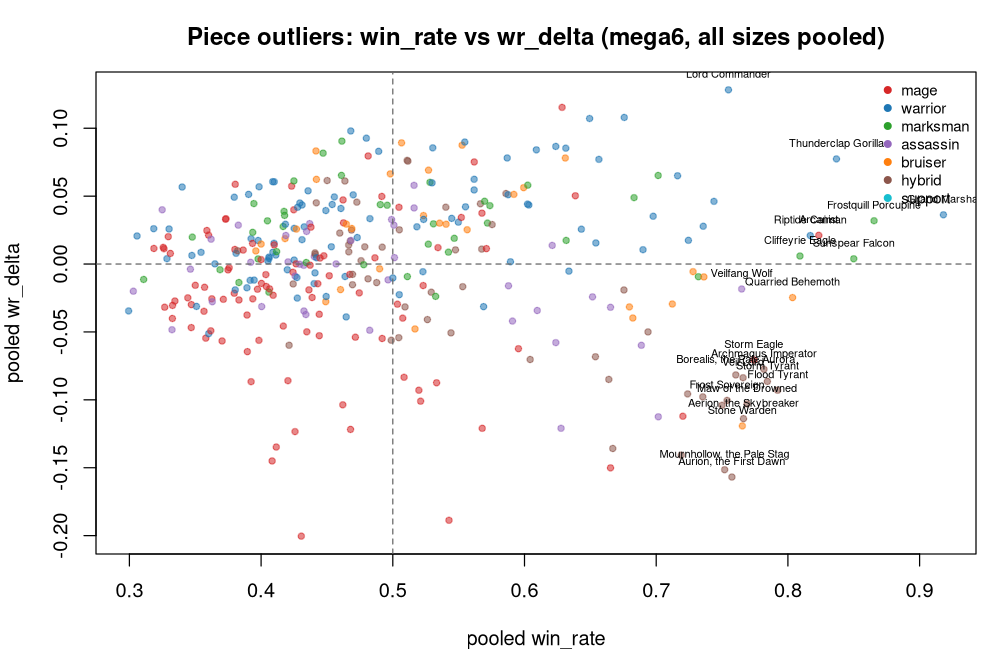
\includegraphics[width=0.86\linewidth,height=0.42\textheight,keepaspectratio]{plots/m6_07_outlier_scatter.png}
\caption*{\small outlier scatter}
\end{figure}


\section*{10. Recommendations}

Ordered by impact/urgency:\\

1. \textbf{Fix L3 mage kit scaling (HIGH).} Company Captain, Hierarch, Glade Heron, Steam Engineer are all −0.13 to −0.20 at L3 but near-neutral at L1. The root cause is that mage levelling bonuses either don't amplify the right stats or the ability-scaling coefficients don't increase correctly with level. Audit \texttt{build\_\allowbreak{}champion\_\allowbreak{}at\_\allowbreak{}level} for mage stat application. This is the single biggest balance gap in the data.\\

2. \textbf{Audit hybrid T10 boss kits (HIGH).} Aurion, Mournhollow, Nerei, Flood Tyrant, Storm Tyrant all carry −0.09 to −0.16 wr\_delta at L3. Boss pieces need to post overwhelming win rates to deliver the designed threat level. Likely a combination of hybrid role complexity and L3 kit scaling.\\

3. \textbf{Nerf Lord Commander L3 and Coral Colossus L3 (MEDIUM).} Both warriors are +0.10--+0.13 over budget at L3. Their L1/L2 numbers are borderline acceptable (Coral Colossus L2 = +0.098 is also high); the L3 ability step appears to give disproportionate power to these specific warriors.\\

4. \textbf{Review bruiser timeout contribution (LOW/MONITORING).} 35\% timeout rate at 8v8 is high. The simulation cap at 12,000 ticks is a design constant but if combat tuning drives it higher, consider raising it. Monitor whether bruiser timeout rate continues to climb as team size grows.\\

5. \textbf{Weather favor: snow affinity may need a small boost (LOW).} Snow is the only ring-affinity with a negative own-weather delta (−0.009 at 2v2 L1). All others show a positive signal. A minor stat-pack adjustment for snow affinity would bring it in line.\\


\section*{11. Mega6 vs mega7 (partial re-run)}

\texttt{results/\allowbreak{}mega\_\allowbreak{}10v10\_\allowbreak{}3/\allowbreak{}} (mega7) ran team2 and team3 before interruption. Team2 data is bit-for-bit identical to mega6. Team3 median matches = 17 vs mega6's 20. No new signal is present. The interrupted re-run confirms that mega6 is stable and reproducible for these stages.\\


\section*{12. Reproducibility}

All scripts at repo root, run in order:\\

\begin{lstlisting}
Rscript reviews/mega_sim/09_mega6.R        # tables + cache_mega6.rds
Rscript reviews/mega_sim/10_mega6_plots.R  # plots/m6_01..m6_08.png
python3 reviews/mega_sim/build_mega6_pdf.py  # mega6_analysis_report.pdf
\end{lstlisting}

Data: \texttt{results/\allowbreak{}mega\_\allowbreak{}10v10\_\allowbreak{}2/\allowbreak{}} (ratings + results CSVs). Baseline: \texttt{results/\allowbreak{}mega\_\allowbreak{}10v10/\allowbreak{}}.\\
R version: 4.5.3. Base R only --- no external packages required.\\

\end{document}